\chapter{Desenvolvimento}

Levando em conta todas as características e opções levantadas no capítulo anterior, é necessário analisar não só quais módulos devem compor as shields, mas principalmente como deve ser a  organização deles para tornar sua utilização realmente relevante.

Antes de iniciar efetivamente com a escolha de módulos e sensores, será apresentada uma lista de requisitos que devem servir de referência em todas as escolhas, já que os requisitos descrevem todas as propriedades a serem atendidas pelo produto.

Além disso, como um dos objetivos deste trabalho, será necessário fazer a escolha do microcontrolador e do hardware que servirá de base para os módulos, da mesma forma para os componentes, esta etapa deverá atender os requisitos do projeto.



\section{Requisitos}

O projeto com um todo deve atender os seguintes requisitos:

\begin{itemize}
	\item A placa de desenvolvimento base deve um modelo que já é utilizado em disciplinas de microcontroladores visando popularizar a utilização das shields desenvolvidas;
	\item Deve conter uma maneira clara de exibir dados, preferencialmente por meio de um display e uma interface mais simples de exibição;
	\item 3 ou mais botões para interação;
	\item 2 ou mais sensores ou módulos com comunicação I2C;
	\item 1 ou mais sensores analógicos;
	\item Driver para controle de 1 ou mais motores;
	\item 1 ou mais padrões de comunicação sem fio;
	\item As shields devem ter dimensões iguais ou muito próximas à da plataforma escolhida.
	
\end{itemize} 

\section{Restrições}

A escolha dos componentes têm alguns restrições que afetam diretamente as opções disponíveis para o desenvolvimento deste trabalho. O tipo de montagem do componente é uma das limitações já que os testes do projeto utilizando componentes no formado SMD (\textit{surface-mount device}) seriam muito mais complexos, além disso, como já citado, serão selecionados apenas componentes e módulos disponíveis no mercado brasileiro visando reduzir custos de prototipagem.

\section{Ferramentas}

Até esta etapa foi utilizado apenas um software para elaboração dos esquemáticos e layouts, o \textit{Eagle}.

Nas próximas etapas, o \textit{Proteus} será o software responsável pela simulação de alguns subcircutos. Além disso, para a programação do microcontrolador será utilizado o \textit{Code Compose Studio} devido a escolha da placa de desenvolvimento, detalhada a seguir.

\section{Proposta}

A proposta em si consiste na elaboração de 4  shields que se adaptam entre si na Launchpad. Idealmente o usuário pode utilizar qualquer quantidade de shields diferentes e na ordem que preferir.

O principal cuidado que foi tomado durante o desenvolvimento foi com relação utilização adequada dos portas do microcontrolador, pois elas são relativamente limitadas. O anexo~\ref{sec:pinout} foi utilizado como principal referência para seleção de portas a serem utilizadas pelos módulos.

\subsection{Placa principal}

Na FGA o microcontrolador utilizado é da Texas Instruments, a empresa conta com uma grande variedade de modelos com diferentes características e funcionalidades, entretanto buscando manter o modelo já utilizado na disciplina será utilizado a família de microcontroladores MSP430.

A Texas Instruments também disponibiliza um grande suporte para o desenvolvimento contando com datasheets detalhados e artigos sobre diversaos funcionalidades de seus produtos, tudo pode ser encontrado em \citeonline{TexasInstruments2019}.

\subsection{MSP430}

Essa linha de produtos tem como principal característica o baixo uso de energia, além disso este conjunto de microntroladores conta suporte a periféricos digitais e analógicos integrados, o que facilita muito o desenvolvimento de projetos em geral.

\subsubsection{LauchPad MSP430}

Launchpad foi o nome dado para o kit de desenvolvimento da Texas Instruments, se trata de uma placa de baixo custo que torna a utilização do microcontrolador muito mais simples, ele conta com pinos para acessar as conexões do chip além de um debugger que faz a conexão e programação do chip através de um cabo USB.

Entre a duas opções utilizada na disciplina de Eletrônica Embarcada, a escolha foi o MSP430F5529 LaunchPad Evaluation Kit (figura \ref{fig:launchpad}) por contar com um maior número de portas disponíveis, característica necessária para atender todos os requisitos.

\begin{figure}[h!]
  \centering
  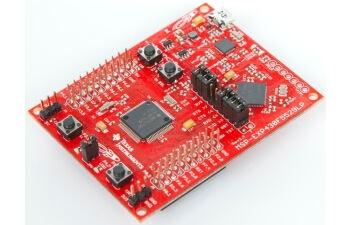
\includegraphics[width=0.7\linewidth]{figuras/launchpad.jpg}
  \caption{LaunchPad Evaluation Kit.}
  \label{fig:launchpad}
\end{figure}

As principais características desse modelo são:

\begin{itemize}
	\item USB 2.0;
	\item Clock de até 25 MHz;
	\item 128KB de memória Flash e 8KB de RAM;
	\item Conversor A/D de 12 bits;
	\item Debugger open source integrado (eZ-FET lite);
	\item Entrada USB como fonte de 5V e 3.3V com conversor DC/DC de alta eficiência.
\end{itemize}

O número e tipo de portas também é outro fator relevante desta Launchpad, ela conta com 35 pinos de uso geral (GPIO), sendo:

\begin{itemize}
	\item 8 com suporte à comparadores;
	\item 12 com suporte à temporizadores;
	\item 4 portas suportando 2 canais I2C;
	\item 9 portas suportando 3 canais SPI;
	\item 2 portas suportando UART.
\end{itemize}

Levando em conta que todos os tipos de comunicação serão utilizadas em apenas 1 canal, temos no total 28 portas disponíveis para a integração dos shields. As portas responsáveis pelos protocolos de comunicação estão representadas na tabela \ref{tab:serial}.

\begin{table}[h!]
\centering
\begin{tabular}{|c|c|c|}
\hline
Porta & \multicolumn{2}{c|}{Periférico} \\ \hline
P3.3  & \multirow{2}{*}{UART}   & TX    \\ \cline{1-1} \cline{3-3} 
P3.4  &                         & RX    \\ \hline
P4.1  & \multirow{2}{*}{I2C}    & SDA   \\ \cline{1-1} \cline{3-3} 
P4.1  &                         & SCL   \\ \hline
P3.0  & \multirow{3}{*}{SPI}    & MOSI  \\ \cline{1-1} \cline{3-3} 
P3.1  &                         & MISO  \\ \cline{1-1} \cline{3-3} 
P3.2  &                         & CLK   \\ \hline
\end{tabular}
\caption{Pinos de comunicação serial.}
\label{tab:serial}
\end{table}

\subsection{Informações}

\subsubsection*{LEDs}

A diferença de especificações entre os LEDs de alto brilho e difusos são mínimas, entretanto na prática a diferença de brilho é bem percetível. Por  conta desse detalhe a escolha será os LEDs de alto brilho.

O uso do LED RGB será feito em apenas uma das shields, a de Interface, já que é nela que deve se centralizar as informações.

\paragraph*{Corrente de saída}

A portas do microntrolador só funcionam de forma estável com saída que utilizem até 15 mA \cite{TexasInstruments2018} , ou seja, para o LEDs e outros módulos que ultrapassem esse limite será necessária a utilização de uma transistor.

Um dos modelos de transistor mais comum é o BC547, que por sua vez atende todas a necessidades desse projeto e portanto será o utilizado para fornecer a corrente não só para os LEDs, mas qualquer outro módulo.

%Assim como no caso de motores, também será necessário um drivers para fornecer a corrente necessária para os componentes, esse driver é o ULN2003A, já especificado na tabela \ref{tab:drivers}.

%Este driver conta com 7 canais, portante será utilizado não só para os LEDs, mas sim para qualquer outro componente que necessite uma corrente superior a 15 mA, limite que já pode gerar instabilidades de tensão \cite{TexasInstruments2018}.


\subsubsection*{Display}

O grande fator limitante na escolha é o tamanho, pois apenas o display Oled \ref{fig:display_oled} é compatível com as dimensões da placa. Embora seja a única opção viável, esse display conseguirá atender praticamente todas as necessidades.

\subsubsection*{Display 7 segmentos}

Como um intermediário, se tratando de complexidade de funcionamento, a shield também deve conter 4 display de 7 segmentos controlados por um conversor BCD-7segmentos (CD4511) e 4 transistores de ativação para o funcionamento por meio de multiplexação.

\subsubsection*{Botões}

Por conta da limitação de espaço serão adicionados apenas 3 botões do tipo push-button SPST (figura \ref{fig:button}) nesta shield, número suficiente para atender o requisitos.

Embora estes botões sejam os mais comuns, eles podem apresentar problemas com debounce, por isso e circuito RC simples foi adicionado ao esquemátivo visando minimizar esses erros.

\subsubsection{Esquemático}

As conexões devem seguir os dados da tabela \ref{tab:interface}.

\begin{table}[h!]
\centering
\begin{tabular}{|c|c|c|c|}
\hline
Porta & \multicolumn{3}{c|}{Periférico}                                           \\ \hline
P2.0  & \multirow{3}{*}{LED RGB}      & \multicolumn{2}{c|}{Vermelho}             \\ \cline{1-1} \cline{3-4} 
P2.2  &                               & \multicolumn{2}{c|}{Verde}                \\ \cline{1-1} \cline{3-4} 
P7.4  &                               & \multicolumn{2}{c|}{Azul}                 \\ \hline
P4.1  & \multirow{2}{*}{Display Oled} & \multirow{2}{*}{I2C}           & SDA      \\ \cline{1-1} \cline{4-4} 
P4.2  &                               &                                & SCL      \\ \hline
P1.5  & \multirow{8}{*}{7 segmentos}  & \multirow{4}{*}{Número}        & Bit 0    \\ \cline{1-1} \cline{4-4} 
P1.4  &                               &                                & Bit 1    \\ \cline{1-1} \cline{4-4} 
P1.3  &                               &                                & Bit 2    \\ \cline{1-1} \cline{4-4} 
P1.2  &                               &                                & Bit 3    \\ \cline{1-1} \cline{3-4} 
P4.3  &                               & \multirow{4}{*}{Multiplexação} & Dígito 1 \\ \cline{1-1} \cline{4-4} 
P4.0  &                               &                                & Dígito 2 \\ \cline{1-1} \cline{4-4} 
P3.7  &                               &                                & Dígito 3 \\ \cline{1-1} \cline{4-4} 
P8.2  &                               &                                & Dígito 4 \\ \hline
P7.0  & \multirow{3}{*}{Botões}       & \multicolumn{2}{c|}{BT0}                  \\ \cline{1-1} \cline{3-4} 
P3.6  &                               & \multicolumn{2}{c|}{BT1}                  \\ \cline{1-1} \cline{3-4} 
P3.5  &                               & \multicolumn{2}{c|}{BT2}                  \\ \hline
\end{tabular}
\caption{Conexões shield de interface}
\label{tab:interface}
\end{table}

O circuito completo está representado no anexo \ref{anx:interface}.

\subsubsection{Modelo PCB}

A organização dos componentes selecionados devem seguir o modelo da figura \ref{fig:interface_pcb}.

\begin{figure}[h!]
  \centering
    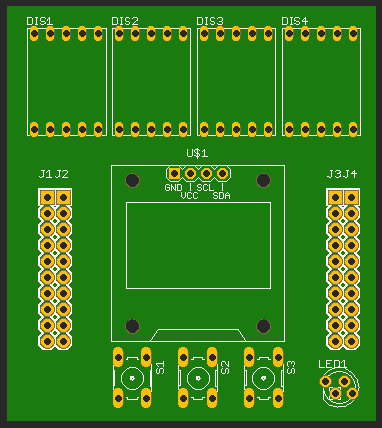
\includegraphics[width=.5\textwidth]{figuras/interface_pcb.png}
    \caption{Modelo da shield de interface} Fonte: Autoria própria
    \label{fig:interface_pcb}
\end{figure}

\subsection{Sensores}

\subsubsection*{Temperatura}

De forma a tornar o projeto mais genérico, o modelo sem contado será o escolhido. Dentre as opções existentes no mercado brasileiro a mais comum e acessível é o DTH11 (figura \ref{fig:dth11}), além disso seu funcionamento é baseado em comunicação \textit{one-wire}, podendo ser uma ótima maneira de explorar as funções do microcontrolador para implantar uma maneira de decodificar os dados recebidos. Vale ressaltar que além de temperatura este sensor também fornece valores de umidade, tornando-o ainda mais versátil.

\subsubsection*{Acelerômetro}

Devida às vantagens já mencionadas na seção \ref{sec:acel}, a escolha para este projeto será o MPU 6050 (figura \ref{fig:display_oled}).

\subsubsection*{Sensor de Luminosidade}

Devida a sua simplicidade, o LDR (figura \ref{fig:ldr}) também deve compor a shield.

\subsubsection*{Sensor Infravermelho}

Não tão simples, e com aplicações bem específicas, o TSOP4838 (figura \ref{fig:infra}) deve integrar o shield para ter um possibilidade extra na elaboração de projetos.

\begin{figure}[h!]
\centering
  \begin{subfigure}[b]{0.3\textwidth}
  \centering
    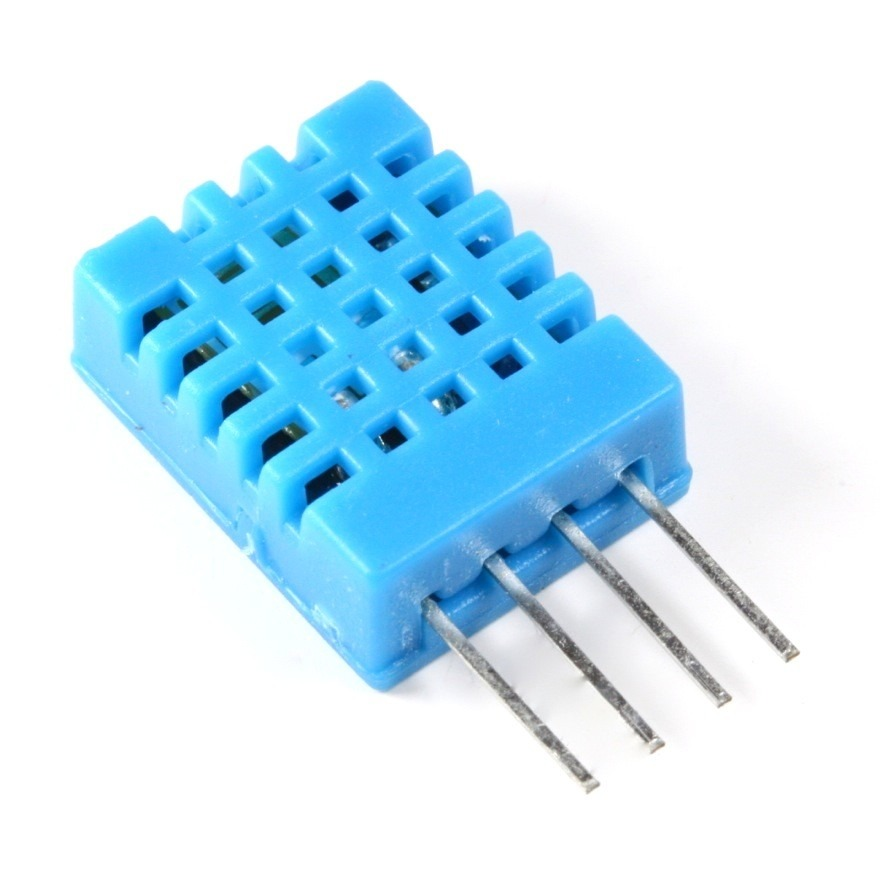
\includegraphics[width=\textwidth]{figuras/dth11.jpg}
    \caption{DTH11} Fonte: \cite{FilipeFlop2019c}
    \label{fig:dth11}
  \end{subfigure}
  %
  \begin{subfigure}[b]{0.3\textwidth}
  \centering
    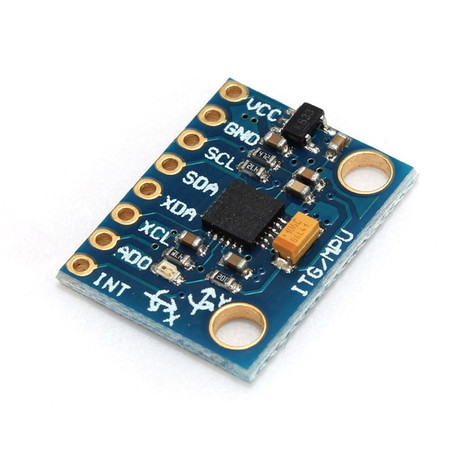
\includegraphics[width=\textwidth]{figuras/mpu6050.jpg}
    \caption{MPU 6050} Fonte: \cite{FilipeFlop2019d}
    \label{fig:mpu6050}
  \end{subfigure}
  %
  \begin{subfigure}[b]{0.3\textwidth}
  \centering
    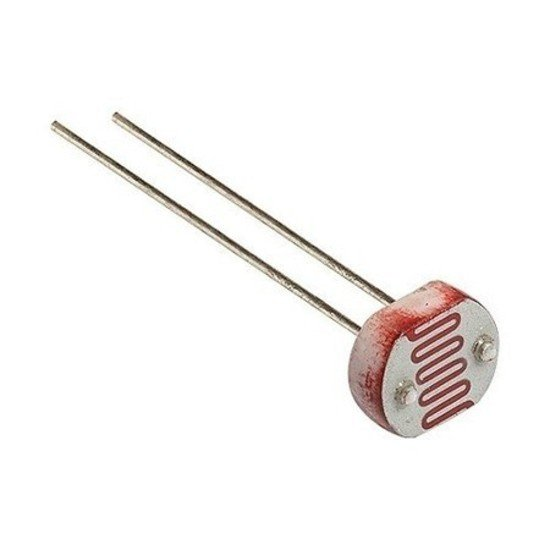
\includegraphics[width=\textwidth]{figuras/ldr.jpg}
    \caption{LDR} Fonte: \cite{EletroGate2019a}
    \label{fig:ldr}
  \end{subfigure}
    %
  \begin{subfigure}[b]{0.3\textwidth}
  \centering
    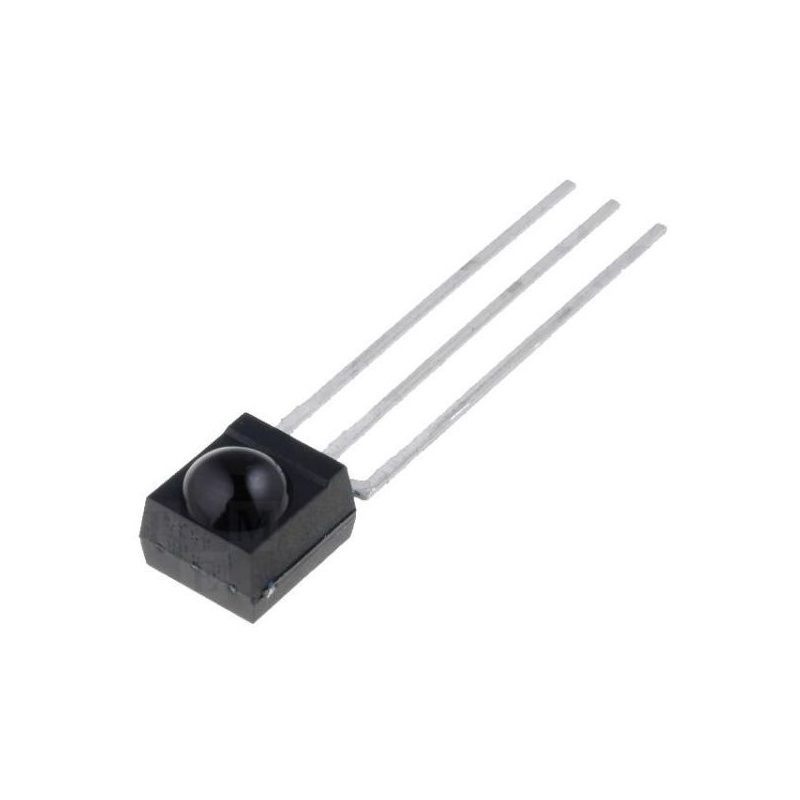
\includegraphics[width=\textwidth]{figuras/infra.jpg}
    \caption{Sensor Infravermelho} Fonte: \cite{FilipeFlop2019e}
    \label{fig:infra}
  \end{subfigure}
 %
  \begin{subfigure}[b]{0.3\textwidth}
  \centering
    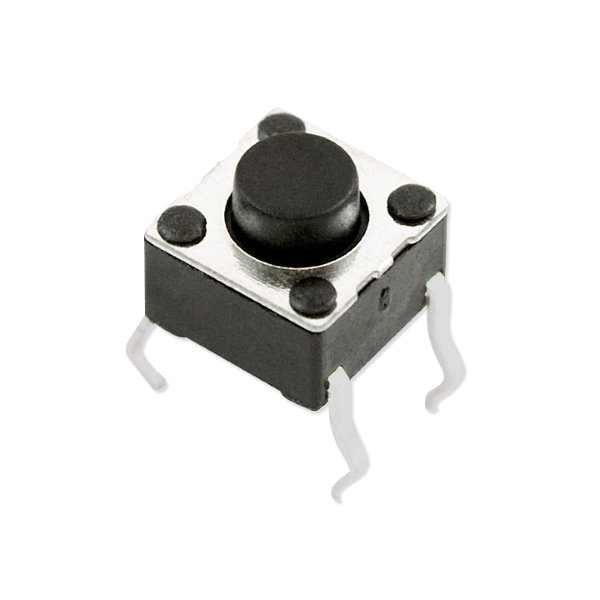
\includegraphics[width=\textwidth]{figuras/button.jpg}
    \caption{Push Button} Fonte: \cite{FilipeFlop2019f}
    \label{fig:button}
  \end{subfigure}
  \caption{Sensores}
\end{figure}

\subsubsection{Esquemático}

As conexões devem seguir os dados da tabela \ref{tab:sensores}.

\begin{table}[h!]
\centering
\begin{tabular}{|c|c|c|}
\hline
Porta & \multicolumn{2}{c|}{Periférico}              \\ \hline
P6.5  & \multicolumn{2}{c|}{LDR}                     \\ \hline
P1.6  & \multicolumn{2}{c|}{Infravermelho}           \\ \hline
P6.6  & \multicolumn{2}{c|}{Temperatura}             \\ \hline
P2.7  & \multirow{3}{*}{Acelerômetro} & Interrupção \\ \cline{1-1} \cline{3-3} 
P4.2  &                               & SCL          \\ \cline{1-1} \cline{3-3} 
P4.1  &                               & SDA          \\ \hline
\end{tabular}
\caption{Conexões shield de sensores.}
\label{tab:sensores}
\end{table}

O circuito completo está representado no anexo \ref{anx:sensor}.

\subsubsection{Modelo PCB}

A organização dos componentes selecionados devem seguir o modelo da figura \ref{fig:sensores_pcb}.

\begin{figure}[h!]
  \centering
    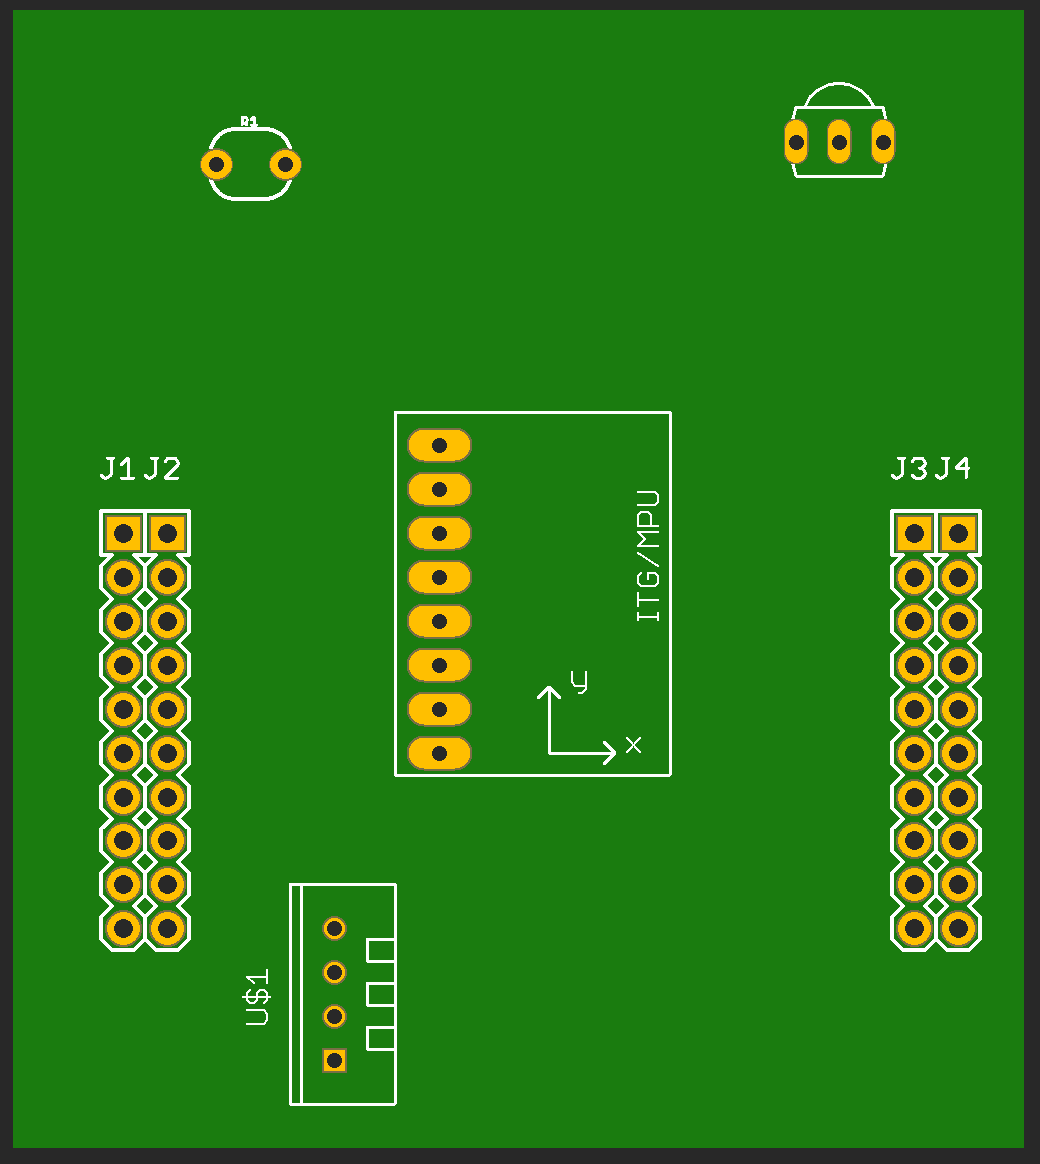
\includegraphics[width=.5\textwidth]{figuras/sensores_pcb.png}
    \caption{Modelo da shield de sensores} Fonte: Autoria própria
    \label{fig:sensores_pcb}
\end{figure}

\subsection{Atuadores}

\subsubsection*{Relé}

A escolha do relé se dá basicamente por conta de sua tensão de operação, 5V no caso deste projeto.

Para seu correto funcionamento e segurança de utilização, é necessária a utilização de um circuito simples de proteção.

\subsubsection*{Driver para Motores}

Conforme mencionado em \ref{sec:duplo}, por conseguir atender o funcionamento de dois tipos de motores e ter boas especificações, o TB6612FNG se torna uma ótima opção para este projeto.

\subsubsection{Esquemático}

As conexões devem seguir os dados da tabela \ref{tab:atuadores}.

\begin{table}[h!]
\centering
\begin{tabular}{|c|c|c|}
\hline
Portas & \multicolumn{2}{c|}{Periférico}           \\ \hline
P6.0   & \multirow{6}{*}{Driver TB6612FNG} & INA1  \\ \cline{1-1} \cline{3-3} 
P6.1   &                                   & INA2  \\ \cline{1-1} \cline{3-3} 
P6.2   &                                   & INB1  \\ \cline{1-1} \cline{3-3} 
P6.3   &                                   & INB2  \\ \cline{1-1} \cline{3-3} 
P2.0   &                                   & PWM A \\ \cline{1-1} \cline{3-3} 
P2.2   &                                   & PWM B \\ \hline
P3.5   & \multicolumn{2}{c|}{Relé}                 \\ \hline
\end{tabular}
\caption{Conexões shield atuadores.}
\label{tab:atuadores}
\end{table}

\subsection{Conectividade}

Por atender perfeitamente os requisitos, a ESP32 será o escolha para ter as conexões Wifi e Bluetooth, entretanto como já temos uma placa de desenvolvimento predefinida faz se necessário apenas as funcionalidade de conectividade sem fio que o ESP32 fornece, portanto neste projeto será utilizado apenas o \textit{core} do kit, o ESP32-WROOM-32, figura \ref{fig:esp32}

\begin{figure}[h!]
  \centering
    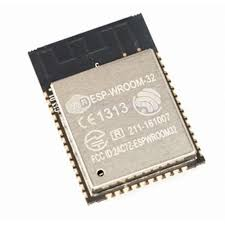
\includegraphics[width=.4\textwidth]{figuras/esp32.jpg}
    \caption{ESP32 Wroom 32} Fonte: \cite{Indiamart2019}
    \label{fig:esp32}
\end{figure}

Para a utilização deste módulo será necessário um circuito auxiliar para a programação do chip \cite{Systems2019}. Além disso será utilizado um firmware específico para o funcionamento por meio de comandos AT \cite{Systems2018}.

As conexões necessárias para a comunicação com a Lauchpad estão na tabela \ref{tab:conect}.

\begin{table}[h!]
\centering
\begin{tabular}{|c|c|c|}
\hline
Porta & \multicolumn{2}{c|}{Periférico}           \\ \hline
P3.4  & \multirow{3}{*}{ESP32-wroom-32} & UART RX \\ \cline{1-1} \cline{3-3} 
P3.3  &                                 & UART TX \\ \cline{1-1} \cline{3-3} 
P3.5  &                                 & Enable  \\ \hline
\end{tabular}
\caption{Conexões shield de conectividade.}
\label{tab:conect}
\end{table}

\section{Cronograma}

As próximas etapas devem seguir o descrito na tabela \ref{tab:cronograma}.


\begin{table}[h!]
\centering
\resizebox{\textwidth}{!}{%
\begin{tabular}{|c|cccc|cccc|cccc|cccc|cccc|cccc|cccc|}
\hline
Atividade                     & \multicolumn{4}{c|}{Jan}                                                          & \multicolumn{4}{c|}{Fev}                                                                                  & \multicolumn{4}{c|}{Mar}                                                                                  & \multicolumn{4}{c|}{Abr}                                                                                  & \multicolumn{4}{c|}{Mai}                                                                                  & \multicolumn{4}{c|}{Jun}                                                                                  & \multicolumn{4}{c|}{Jul}          \\ \hline
Compra dos módulos e sensores &  & \cellcolor[HTML]{3166FF} &                          &                          &                          &                          &                          &                          &                          &                          &                          &                          &                          &                          &                          &                          &                          &                          &                          &                          &                          &                          &                          &                          &                          &  &  &  \\ \hline
Simulação dos subcircuitos    &  &                          & \cellcolor[HTML]{3166FF} & \cellcolor[HTML]{3166FF} &                          &                          &                          &                          &                          &                          &                          &                          &                          &                          &                          &                          &                          &                          &                          &                          &                          &                          &                          &                          &                          &  &  &  \\ \hline
Elaboração dos layouts        &  &                          &                          & \cellcolor[HTML]{3166FF} & \cellcolor[HTML]{3166FF} &                          &                          &                          &                          &                          &                          &                          &                          &                          &                          &                          &                          &                          &                          &                          &                          &                          &                          &                          &                          &  &  &  \\ \hline
Teste dos módulos e sensores  &  &                          &                          &                          & \cellcolor[HTML]{3166FF} & \cellcolor[HTML]{3166FF} &                          &                          &                          &                          &                          &                          &                          &                          &                          &                          &                          &                          &                          &                          &                          &                          &                          &                          &                          &  &  &  \\ \hline
Elaboração do firmware        &  &                          &                          &                          &                          & \cellcolor[HTML]{3166FF} & \cellcolor[HTML]{3166FF} & \cellcolor[HTML]{3166FF} & \cellcolor[HTML]{3166FF} & \cellcolor[HTML]{3166FF} &                          &                          &                          &                          &                          &                          &                          &                          &                          &                          &                          &                          &                          &                          &                          &  &  &  \\ \hline
Elaboração da documentação    &  &                          &                          &                          &                          &                          &                          & \cellcolor[HTML]{3166FF} & \cellcolor[HTML]{3166FF} & \cellcolor[HTML]{3166FF} & \cellcolor[HTML]{3166FF} & \cellcolor[HTML]{3166FF} &                          &                          &                          &                          &                          &                          &                          &                          &                          &                          &                          &                          &                          &  &  &  \\ \hline
Correções nos layouts         &  &                          &                          &                          &                          &                          &                          &                          &                          &                          &                          &                          & \cellcolor[HTML]{3166FF} & \cellcolor[HTML]{3166FF} &                          &                          &                          &                          & \cellcolor[HTML]{3166FF} & \cellcolor[HTML]{3166FF} &                          &                          &                          &                          &                          &  &  &  \\ \hline
Pedido das PCIs               &  &                          &                          &                          &                          &                          &                          &                          &                          &                          &                          &                          &                          & \cellcolor[HTML]{3166FF} &                          &                          &                          &                          &                          & \cellcolor[HTML]{3166FF} &                          &                          &                          &                          &                          &  &  &  \\ \hline
Testes da placas              &  &                          &                          &                          &                          &                          &                          &                          &                          &                          &                          &                          &                          &                          &                          &                          & \cellcolor[HTML]{3166FF} & \cellcolor[HTML]{3166FF} &                          &                          &                          &                          & \cellcolor[HTML]{3166FF} &                          &                          &  &  &  \\ \hline
Documentação dos resultados   &  &                          &                          & \cellcolor[HTML]{3166FF} &                          & \cellcolor[HTML]{3166FF} &                          &                          &                          & \cellcolor[HTML]{3166FF} & \cellcolor[HTML]{3166FF} & \cellcolor[HTML]{3166FF} &                          &                          & \cellcolor[HTML]{3166FF} & \cellcolor[HTML]{3166FF} &                          &                          &                          &                          & \cellcolor[HTML]{3166FF} & \cellcolor[HTML]{3166FF} &                          & \cellcolor[HTML]{3166FF} &                          &  &  &  \\ \hline
Revisão do documento          &  &                          &                          &                          &                          &                          &                          &                          &                          &                          &                          &                          &                          &                          &                          &                          &                          &                          &                          &                          &                          &                          &                          & \cellcolor[HTML]{3166FF} &                          &  &  &  \\ \hline
Elaboração da apresentação    &  &                          &                          &                          &                          &                          &                          &                          &                          &                          &                          &                          &                          &                          &                          &                          &                          &                          &                          &                          &                          &                          & \cellcolor[HTML]{3166FF} & \cellcolor[HTML]{3166FF} &                          &  &  &  \\ \hline
Apresentação                  &  &                          &                          &                          &                          &                          &                          &                          &                          &                          &                          &                          &                          &                          &                          &                          &                          &                          &                          &                          &                          &                          &                          &                          & \cellcolor[HTML]{3166FF} &  &  &  \\ \hline
\end{tabular}%
}
\caption{Cronograma.}
\label{tab:cronograma}
\end{table}




